Finally, some experiments were conducted in order to compare the three models in different scenarios, all of which are related to luggage distribution as this seemed to be the most interesting efficiency factor.

\section{Different Luggage Distribution}
Apart from the original scenario, in which 19 passengers had 0 luggage, 80 passengers had just 1 luggage, and 21 passengers had 2 luggages, the data set "1LuggagePerPassenger\_2Only2" was tried out for the three models: 0 passengers had 0 luggage, 118 passengers had just 1 luggage and 2 passengers had 2 luggages. The results were arranged into the following table:

\begin{table}[H]
  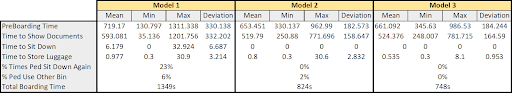
\includegraphics[width=1.0\textwidth]{tables/statistics3.png}
  \caption{Time Statistics - Scenario 1}
  \label{tbl:statistics3}
\end{table}

As suspected in Section 6, where Models 1 and 2 were compared based on the original dataset, the one performance metric for which Model 1 had a better result had indeed been due to chance, and not a specific more efficient feature of Model 1. Now that the amount of luggage each passenger carries has changed, the situation has turned out to be one where passengers spend, on average, 0.8 seconds storing their luggage in Model 2 and 0.977 seconds in Model 1, and where only 2\% of the passengers have to search for a different bin in Model 2, instead of 6\% in Model 1. Unsurprisingly, Model 3 maintains the highest efficiency result in most performance metrics.

\section{Concentration of luggage in a specific area of the plane}
Additionally, two other situations were tested, this time only for Model 1 and Model 2. In the first one (data set "ConcentrateLuggageBack"), the majority of luggage was carried by passengers seated at the back of the airplane, while in the second scenario (data set "ConcentrateLuggageFront"), the luggage was mostly assigned to bins at the front of the airplane. By comparing the performance metrics presented in the tables below with the results obtained in the original scenario, it can be immediately noticed that almost everything remained the same except for the luggage time. For both cases, passengers take much more time to store their belongings as the luggage is unevenly distributed among the bins. This is true for both models.

\begin{table}[H]
  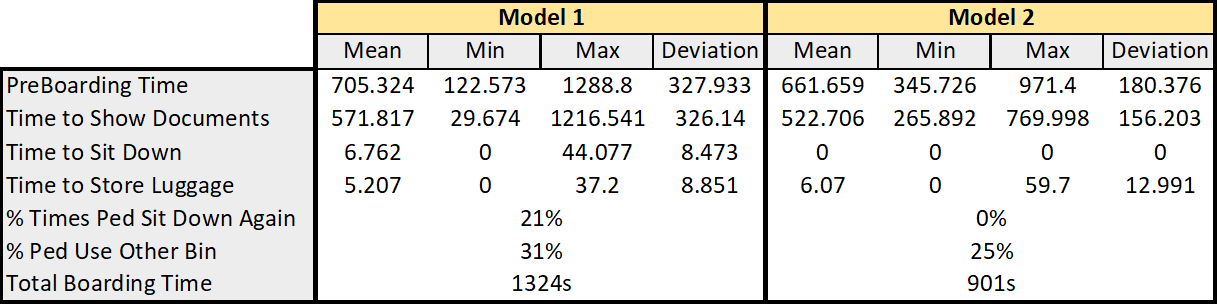
\includegraphics[width=1.0\textwidth]{tables/statistics4.png}
  \caption{Time Statistics - Scenario 2}
  \label{tbl:statistics4}
\end{table}

\begin{table}[H]
  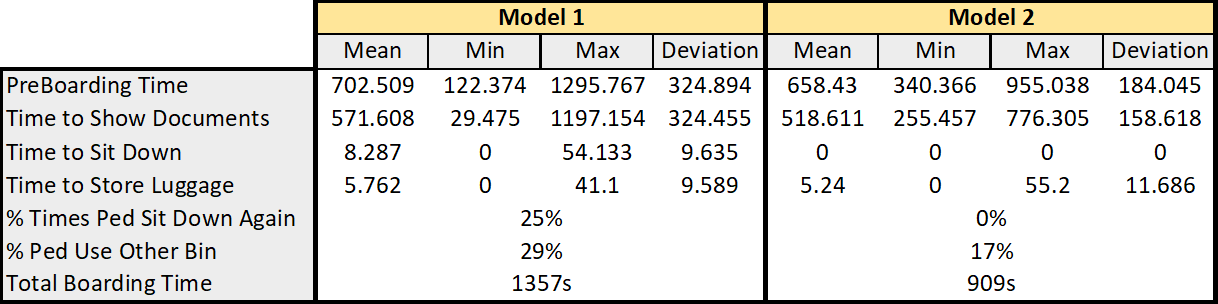
\includegraphics[width=1.0\textwidth]{tables/statistics5.png}
  \caption{Time Statistics - Scenario 3}
  \label{tbl:statistics5}
\end{table}	


